% coucou

\section{Results}

%Faire un FLM n'induit pas que ce n'est pas n'importe quoi. Ce qu'on dit c'est que ne pas faire de FLM alors on a des biais !

\subsection{Pressurized Water Reactor}

\subsubsection{Output analyses}
Figure~\ref{fig:PWR_MOX_FLM_Pu} presents the plutonium fraction at BOC predicted by each FLM and the plutonium fraction at EOC deduced by each software. As all FLM are different, the BOC plutonium fractions differ from a software from another. The wider prediction is given by the CLASS code that predicts plutonium fraction from 4\% until more that 15\%. This range is a direct consequence of the plutonium sampling used for this work. 15\% is clearly unrealistic but some of the plutonium isotopic composition sampled are not either by containing a low amount of fissile. That's why the FLMs may reach such high values.    

\begin{figure}[h]
	\begin{center}
		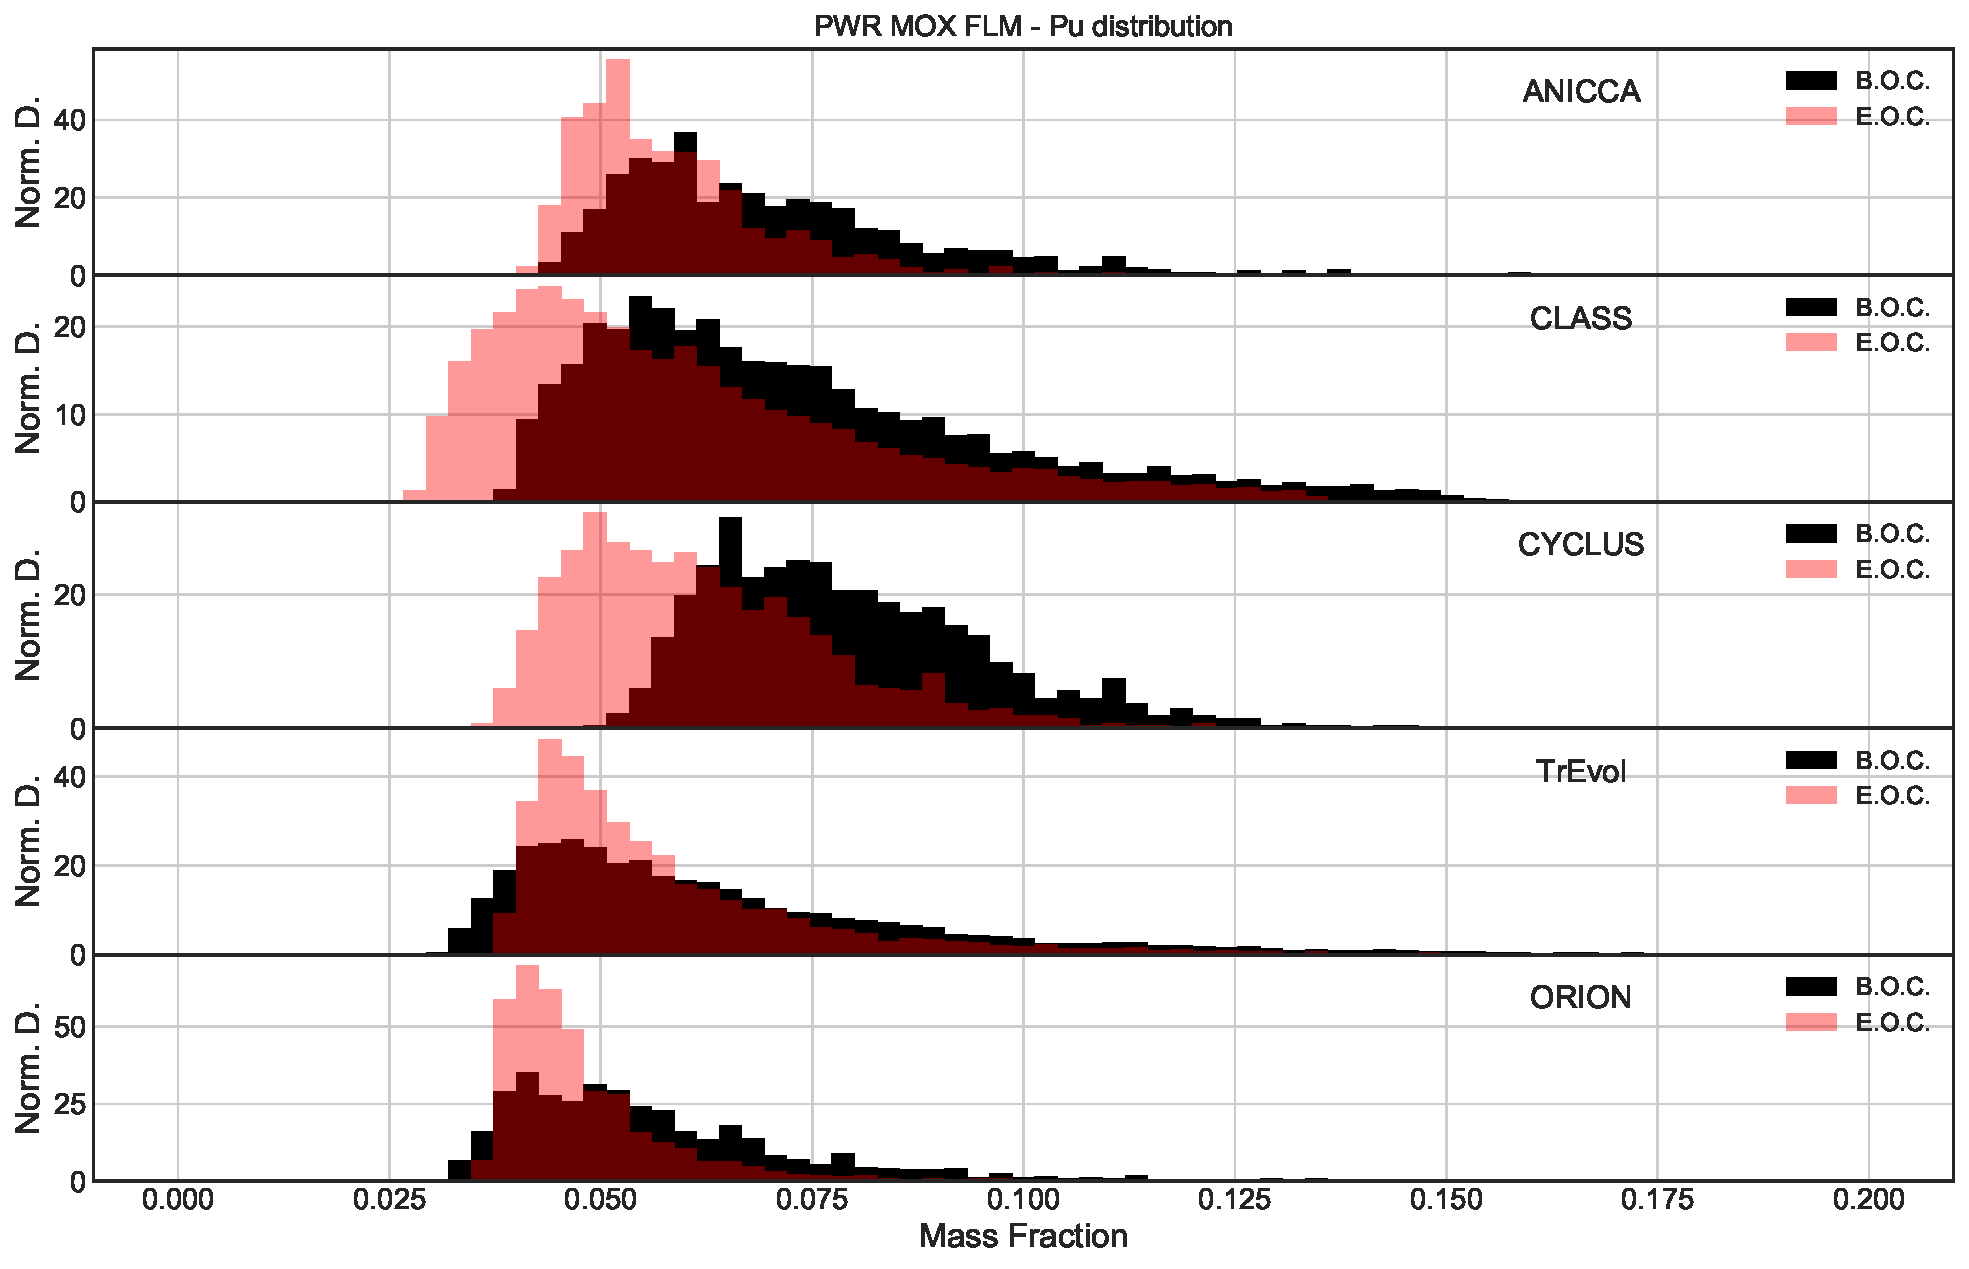
\includegraphics[width = 0.99\textwidth]{../../Feature_1/RAW_DATA/FIG/PWR_MOX_FLM_Pu.pdf}
		\caption{Code outputs for PWR scenario's calculations}
		\label{fig:PWR_MOX_FLM_Pu}
	\end{center}
\end{figure}

The EOC plutonium fraction is clearly shifted to the lower values, proving that plutonium is consumed during irradiation like it should be in PWRs. For ANICCA and for TrEVOL    

\subsubsection{Estimator's calculation}

Figure~\ref{fig:Est1_PWR}, figure~\ref{fig:Est2_PWR} and figure~\ref{fig:Est3_PWR} presents the calculation results for PWR of the different estimators defined in the previous section. 

\paragraph{Plutonium fraction at BOC}
Estimator 1 aims to quantify bias introduced by the use of a FF model on the plutonium enrichment calculation for fresh fuel. It measures the amount of plutonium taken from UOX spent fuel for MOX fuel fabrication. An important positive bias means that the FF model underestimate the mass of spent UOX fuel that has to be processed for the MOX fuel fabrication. As the FF was tuned on a classical plutonium composition, in the middle of the isotopic space available for sampling, Figure~\ref{fig:Est1_PWR} presents some histograms more or less centered on 0.

% Estimateur 2 c'est une estimation de l'inventaire total ! Si on a n'a pas de FLM alors y peut y avoir un impact assez faible pour certain code et important pour d'autre. Il est donc impossible de conclure sur le rôle du FLM pour l'estimateur globaux !         

\begin{figure}[h]
	\begin{center}
		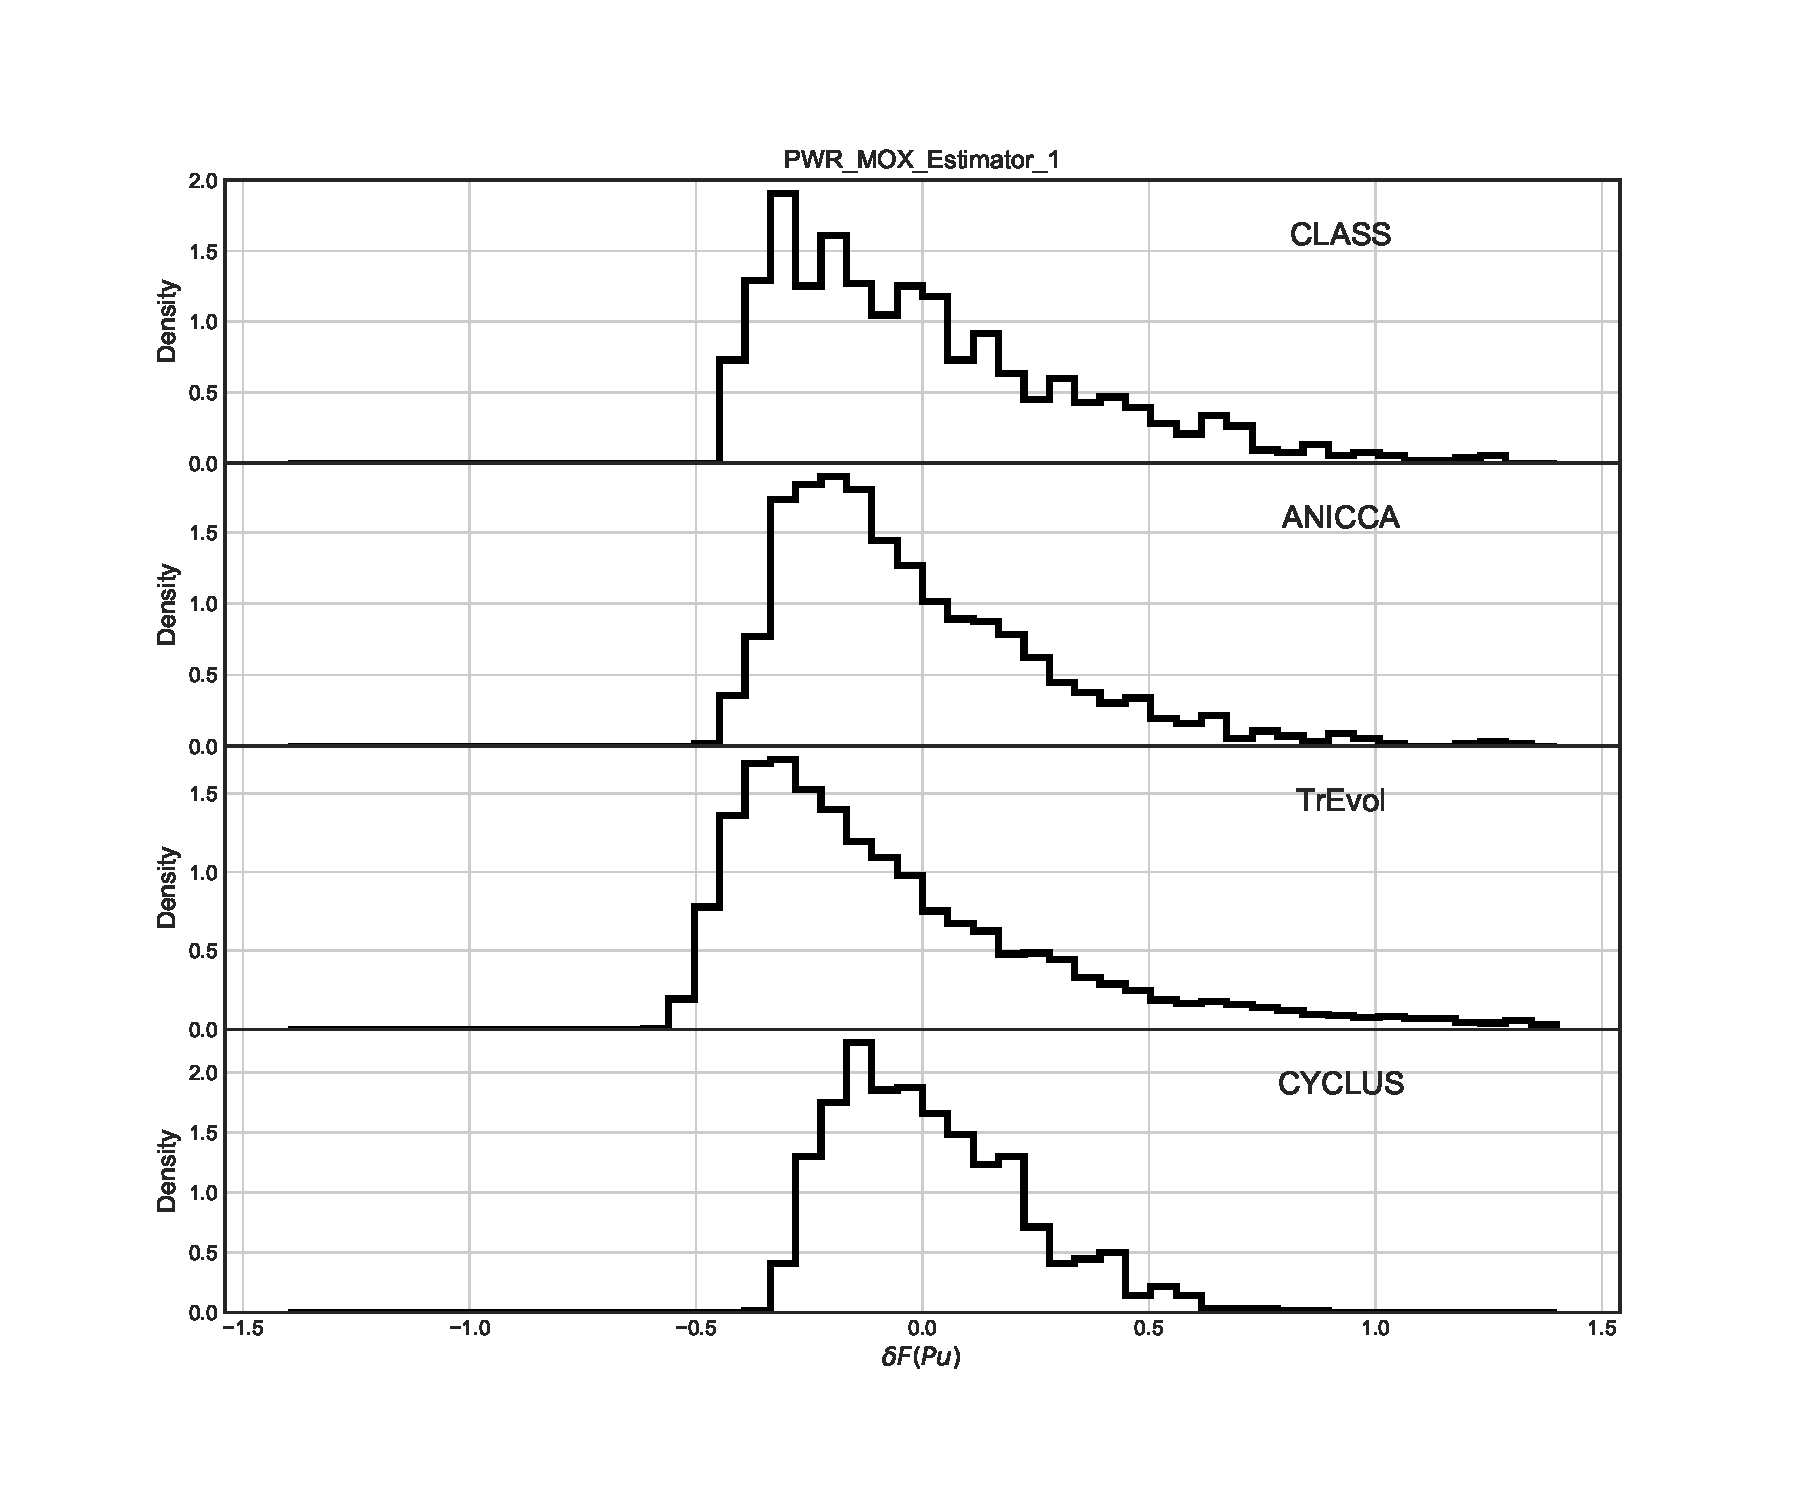
\includegraphics[width = 0.99\textwidth]{../../Feature_1/RAW_DATA/FIG/PWR_MOX_Estimator_1.pdf}
		\caption{Estimator 1 for PWR calculated with ANICCA, CLASS, CYCLUS and TrEVOL}
		\label{fig:Est1_PWR}
	\end{center}
\end{figure}

The standard deviation of the distribution is also a relevant quantity as it quantifies the dispersion of the calculation bias. A small standard deviation implies a narrow distribution and means small calculation biases due to the use of FF model. As we can see on the plot, none of the used software for this work shows a small standard deviation. This means that, in the range of the plutonium composition sampled, the use of a FF model induce strong calculation bias in the fresh MOX fuel plutonium fraction, hence strong bias in the mass of spent fuel that have to be reprocessed for the MOX fuel fabrication.

\paragraph{Ratio between plutonium consumption and plutonium at BOC}
Estimator 2 aims to quantify the amount of plutonium consumption regarding the plutonium mass at BOC. It measures the proportion of plutonium which is burnt during irradiation. Figure~\ref{fig:Est2_PWR} represents the different histograms of this estimator for the 4 codes used in this work. We can clearly see that the use of a FF model for plutonium enrichment calculation leads to strong biases for plutonium consumption. CLASS and CYCLUS  
\begin{figure}[h]
	\begin{center}
		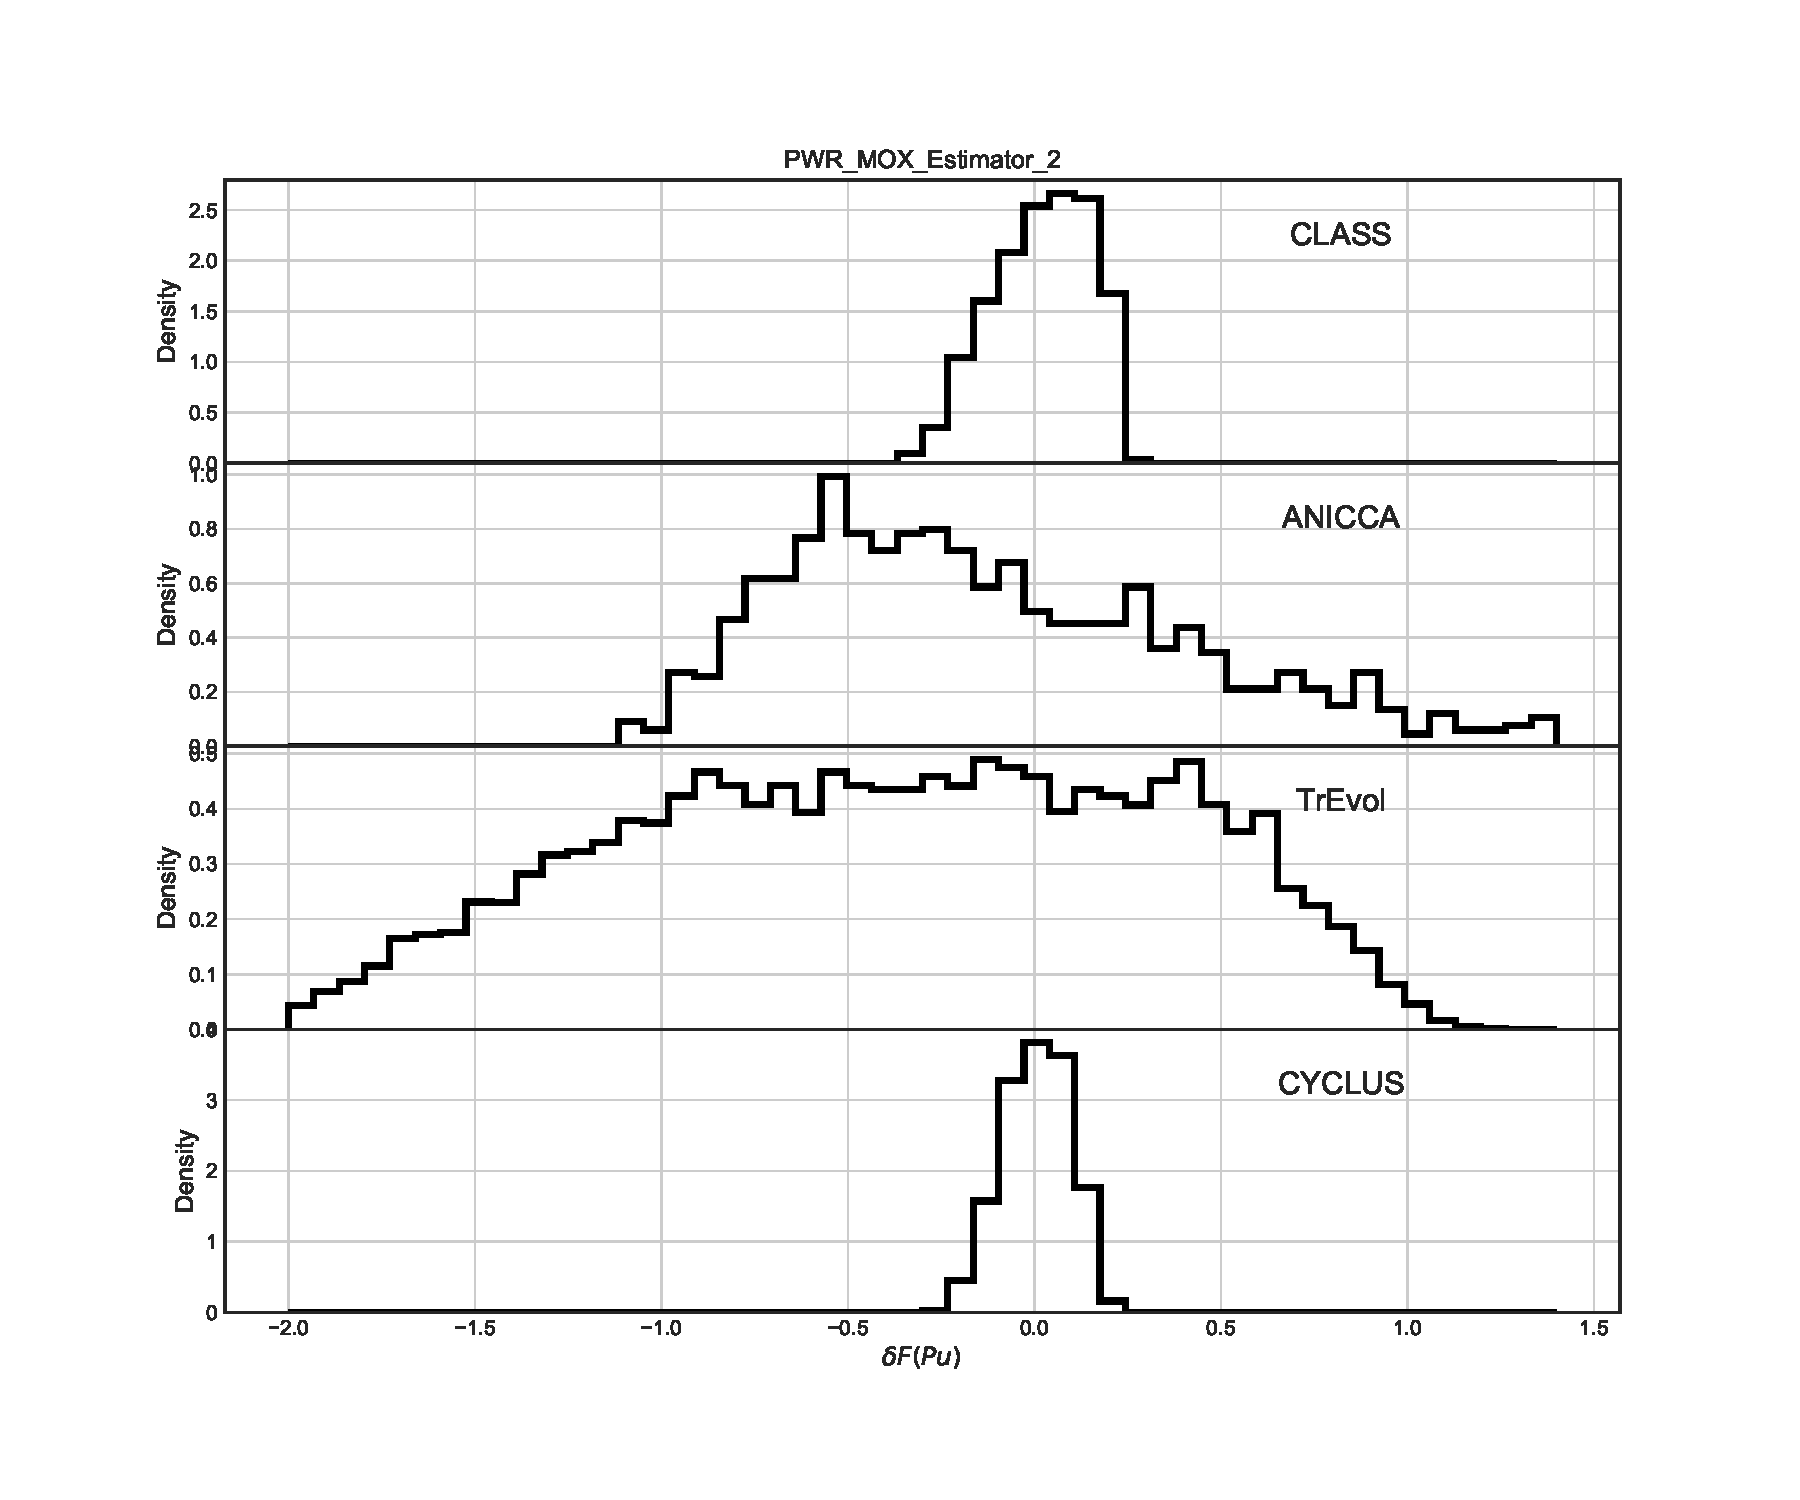
\includegraphics[width = 0.99\textwidth]{../../Feature_1/RAW_DATA/FIG/PWR_MOX_Estimator_2.pdf}
		\caption{Estimator 2 for PWR calculated with CLASS, CYCLUS and TrEVOL}
		\label{fig:Est2_PWR}
	\end{center}
\end{figure}


\paragraph{Plutonium consumption rate}
\begin{figure}[h]
	\begin{center}
		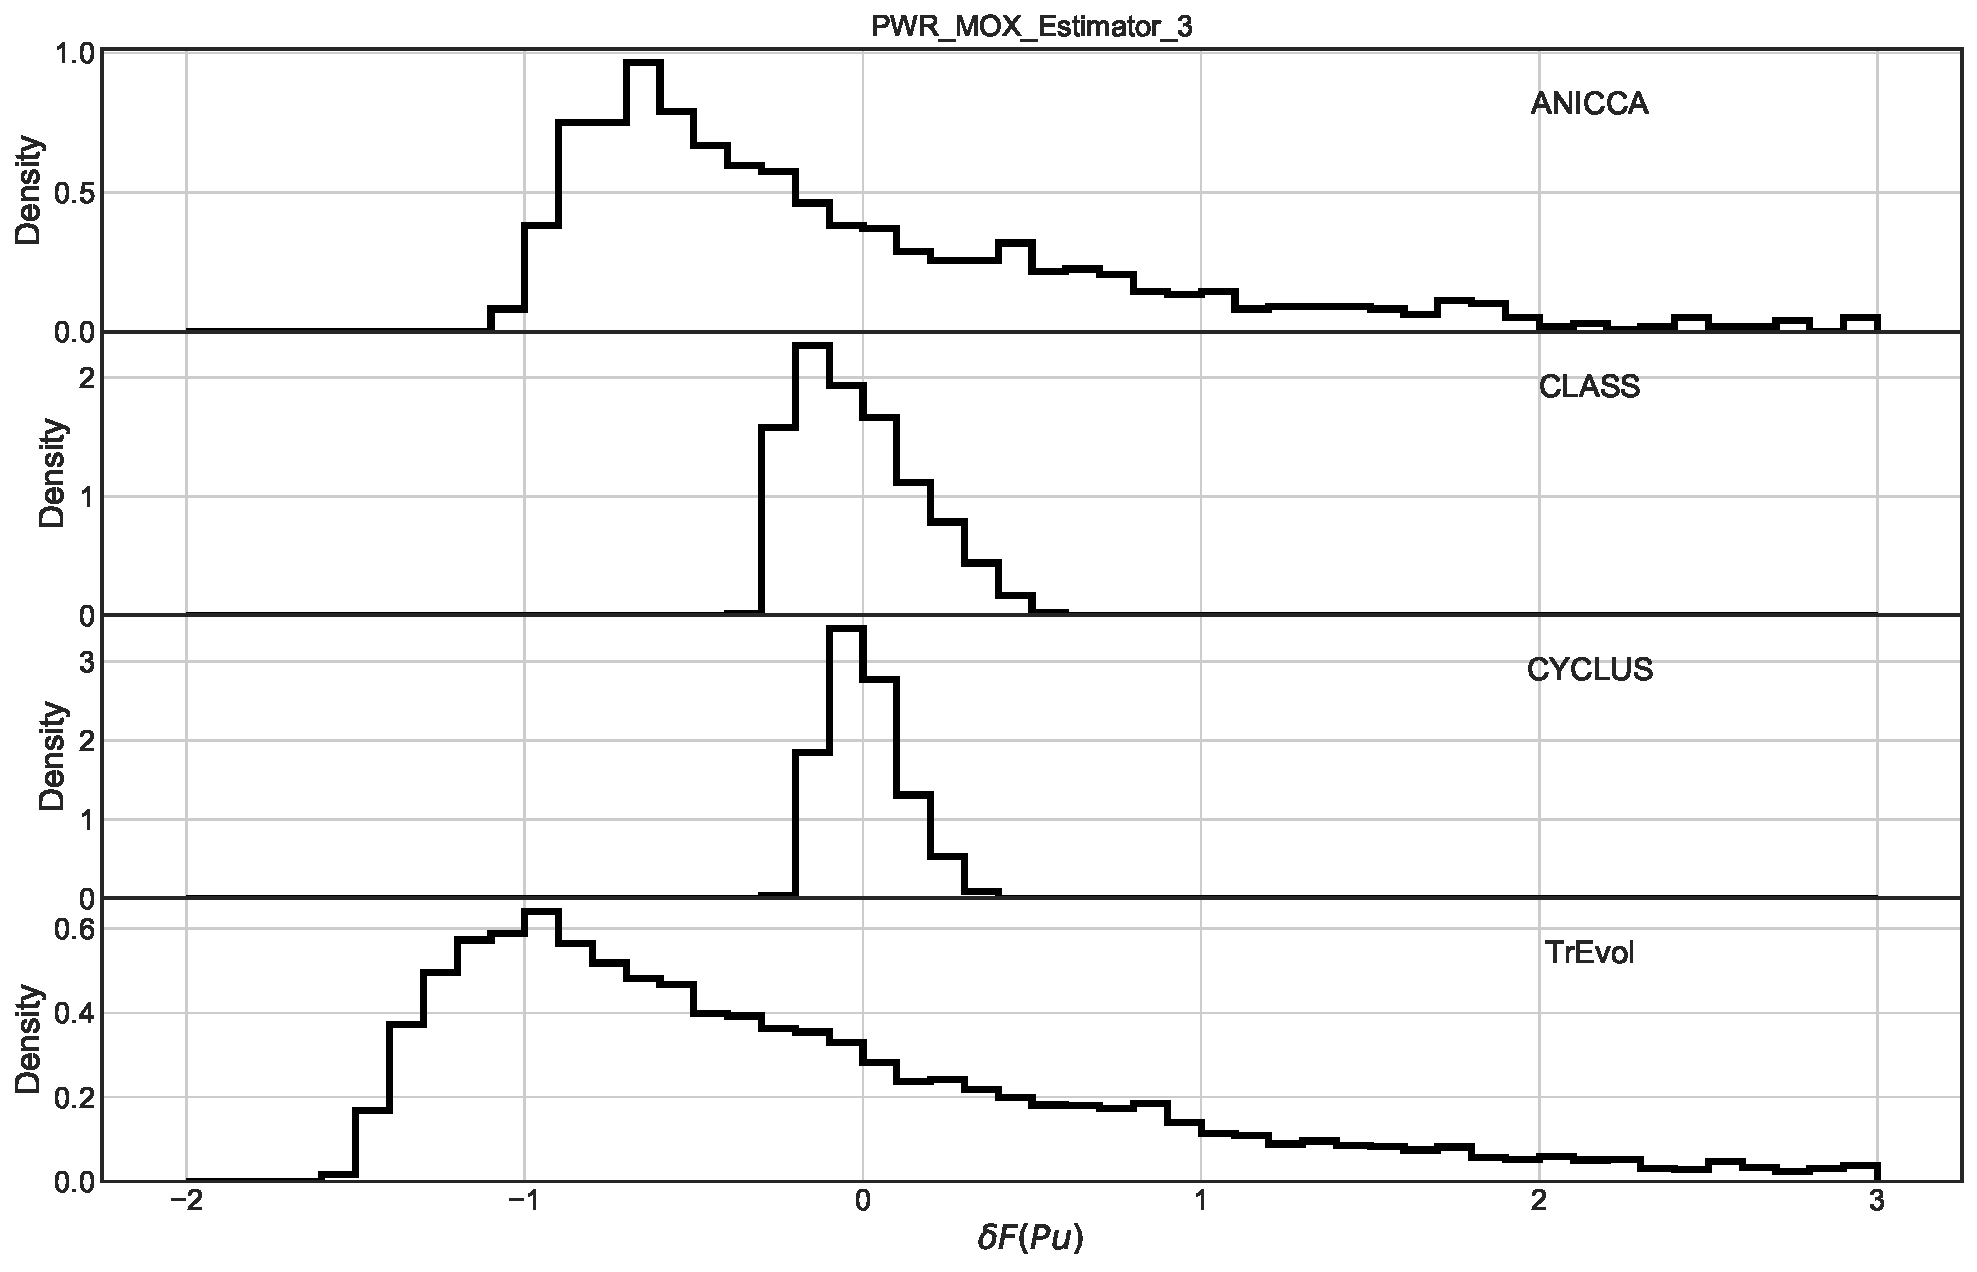
\includegraphics[width = 0.99\textwidth]{../../Feature_1/RAW_DATA/FIG/PWR_MOX_Estimator_3.pdf}
		\caption{Estimator 3 for PWR calculated with CLASS, CYCLUS and TrEVOL}
		\label{fig:Est3_PWR}
	\end{center}
\end{figure}


\paragraph{Discussion}
% Analyse Huge impact, pas forcément remise en cause de la qualité des codes parce que les codes sont utilisés au délà des limites de validités en isotopie Pu.  
% Vecteur super large -> impact faible est encore plus faible en vrai ! 
% Comme la dépletion fait nimp, on ne mesure pas l'effet du FLM et on ne peut pas conclure 

\subsection{Fast Sodium cooled Reactor}

Figure~\ref{fig:Est1_SFR} represents the estimator 1 calculated for Sodium Cooled Fast Reactors calculated with JOSETTE, TrEVOL and CLASS. Like for PWR, it shows the relative difference of plutonium enrichment with the use of a FLM in regards to a FF. Standard deviations of the difference distribution is given in Table~\ref{table:Est1Dev_SFR} for the different codes. 
All codes are in agreement even if CLASS slightly underestimate the FF impact on the plutonium needed for a SFR. The typical biais produced by the use of a FF is smaller than 25\% and is much lower than for PWR.  

\begin{figure}[h]
	\begin{center}
		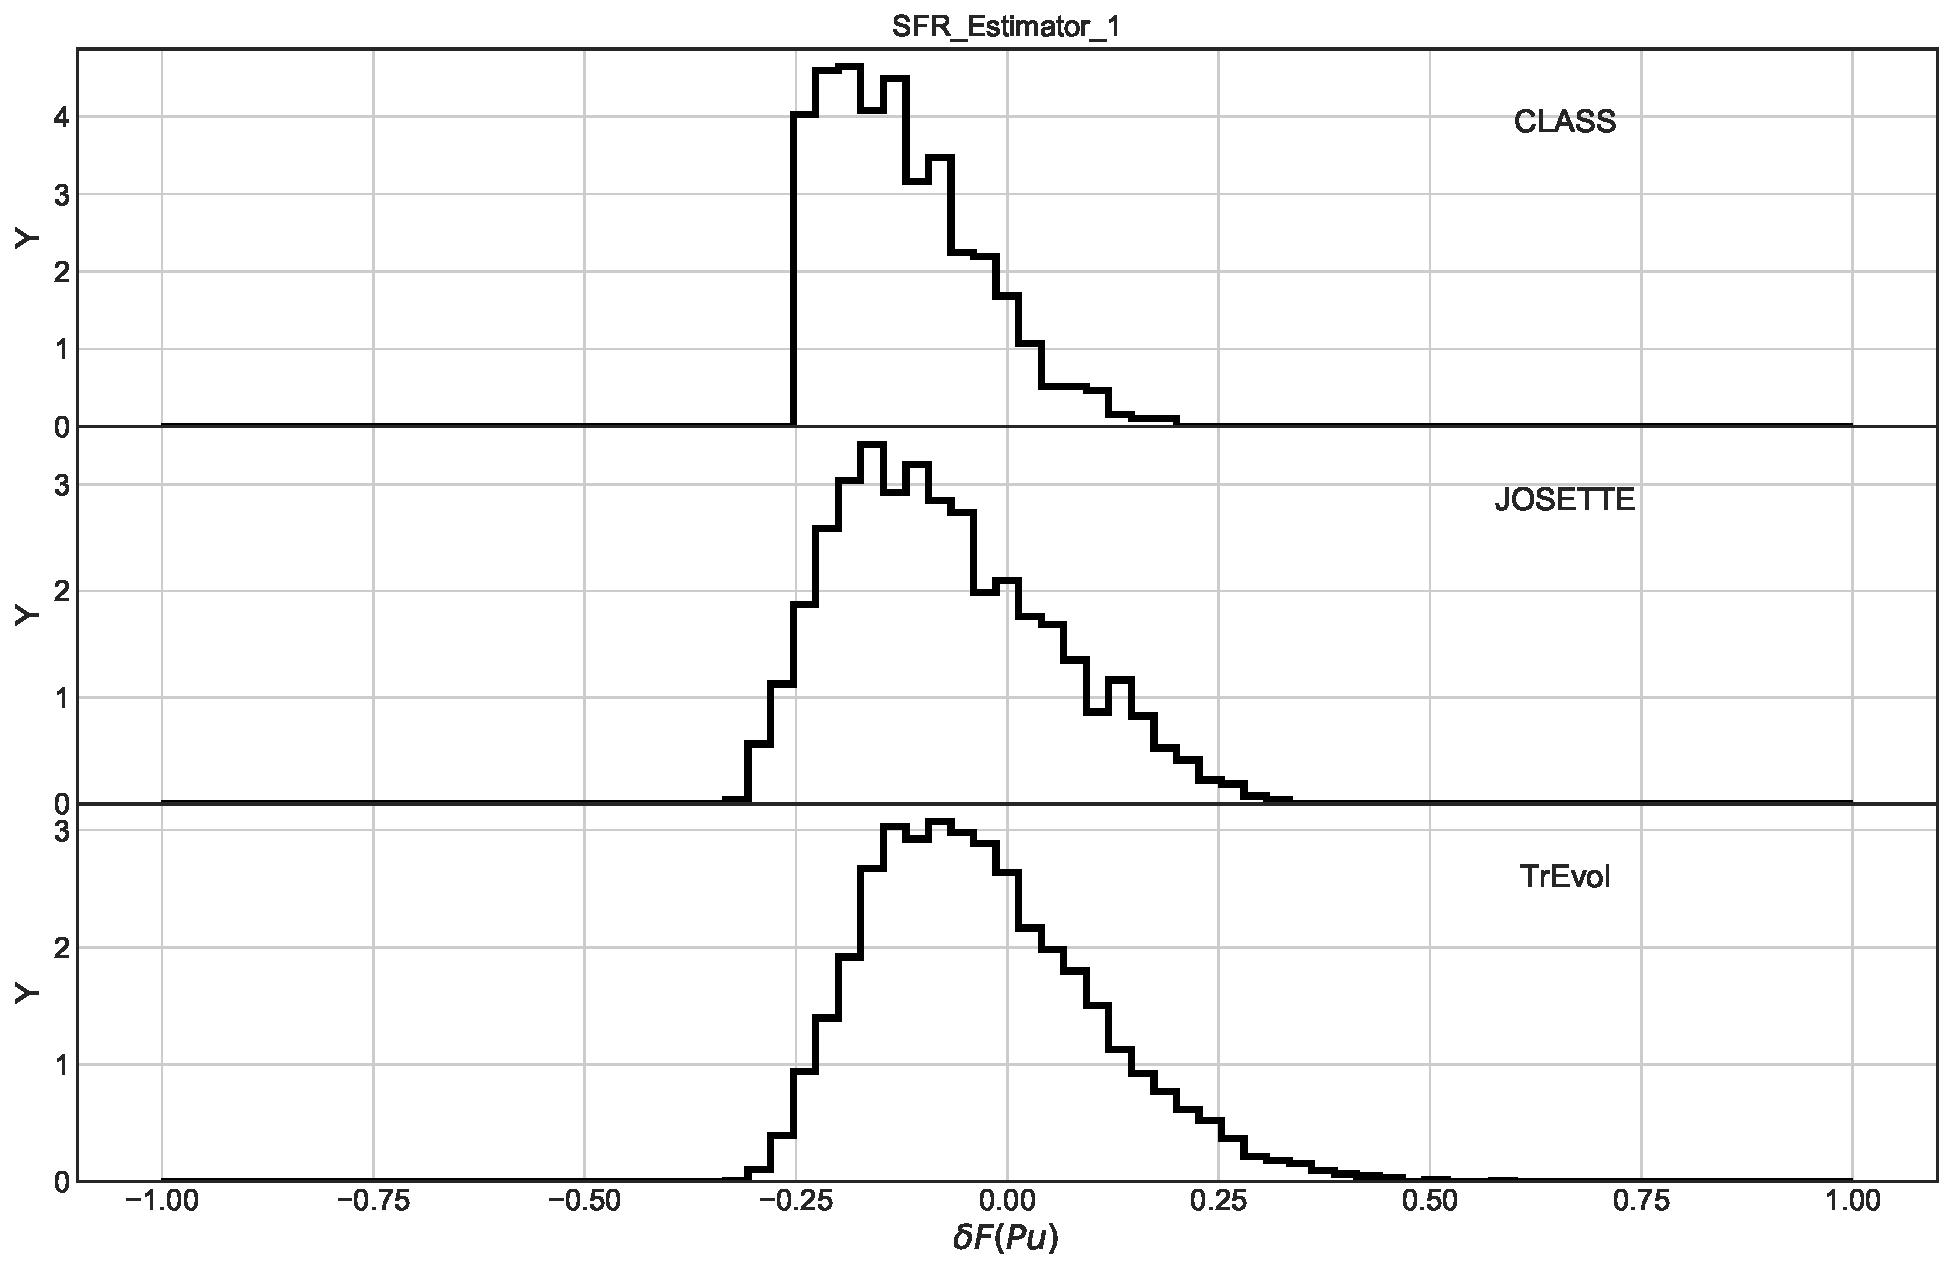
\includegraphics[width = 0.99\textwidth]{../../Feature_1/RAW_DATA/FIG/SFR_Estimator_1.pdf}
		\caption{Estimator 1 for SFR calculated with JOSETTE, TrEVOL, and CLASS}
		\label{fig:Est1_SFR}
	\end{center}
\end{figure}

\begin{table}[h]
	\begin{center}
		\begin{tabular}{|c||c||c|}
			\hline 
				JOSETTE & TrEVOL & CLASS \\
			\hline
				XX & YY & ZZ \\
		\end{tabular}
	\end{center}
	\label{table:Est1Dev_SFR}
\end{table}

\begin{figure}[h]
	\begin{center}
		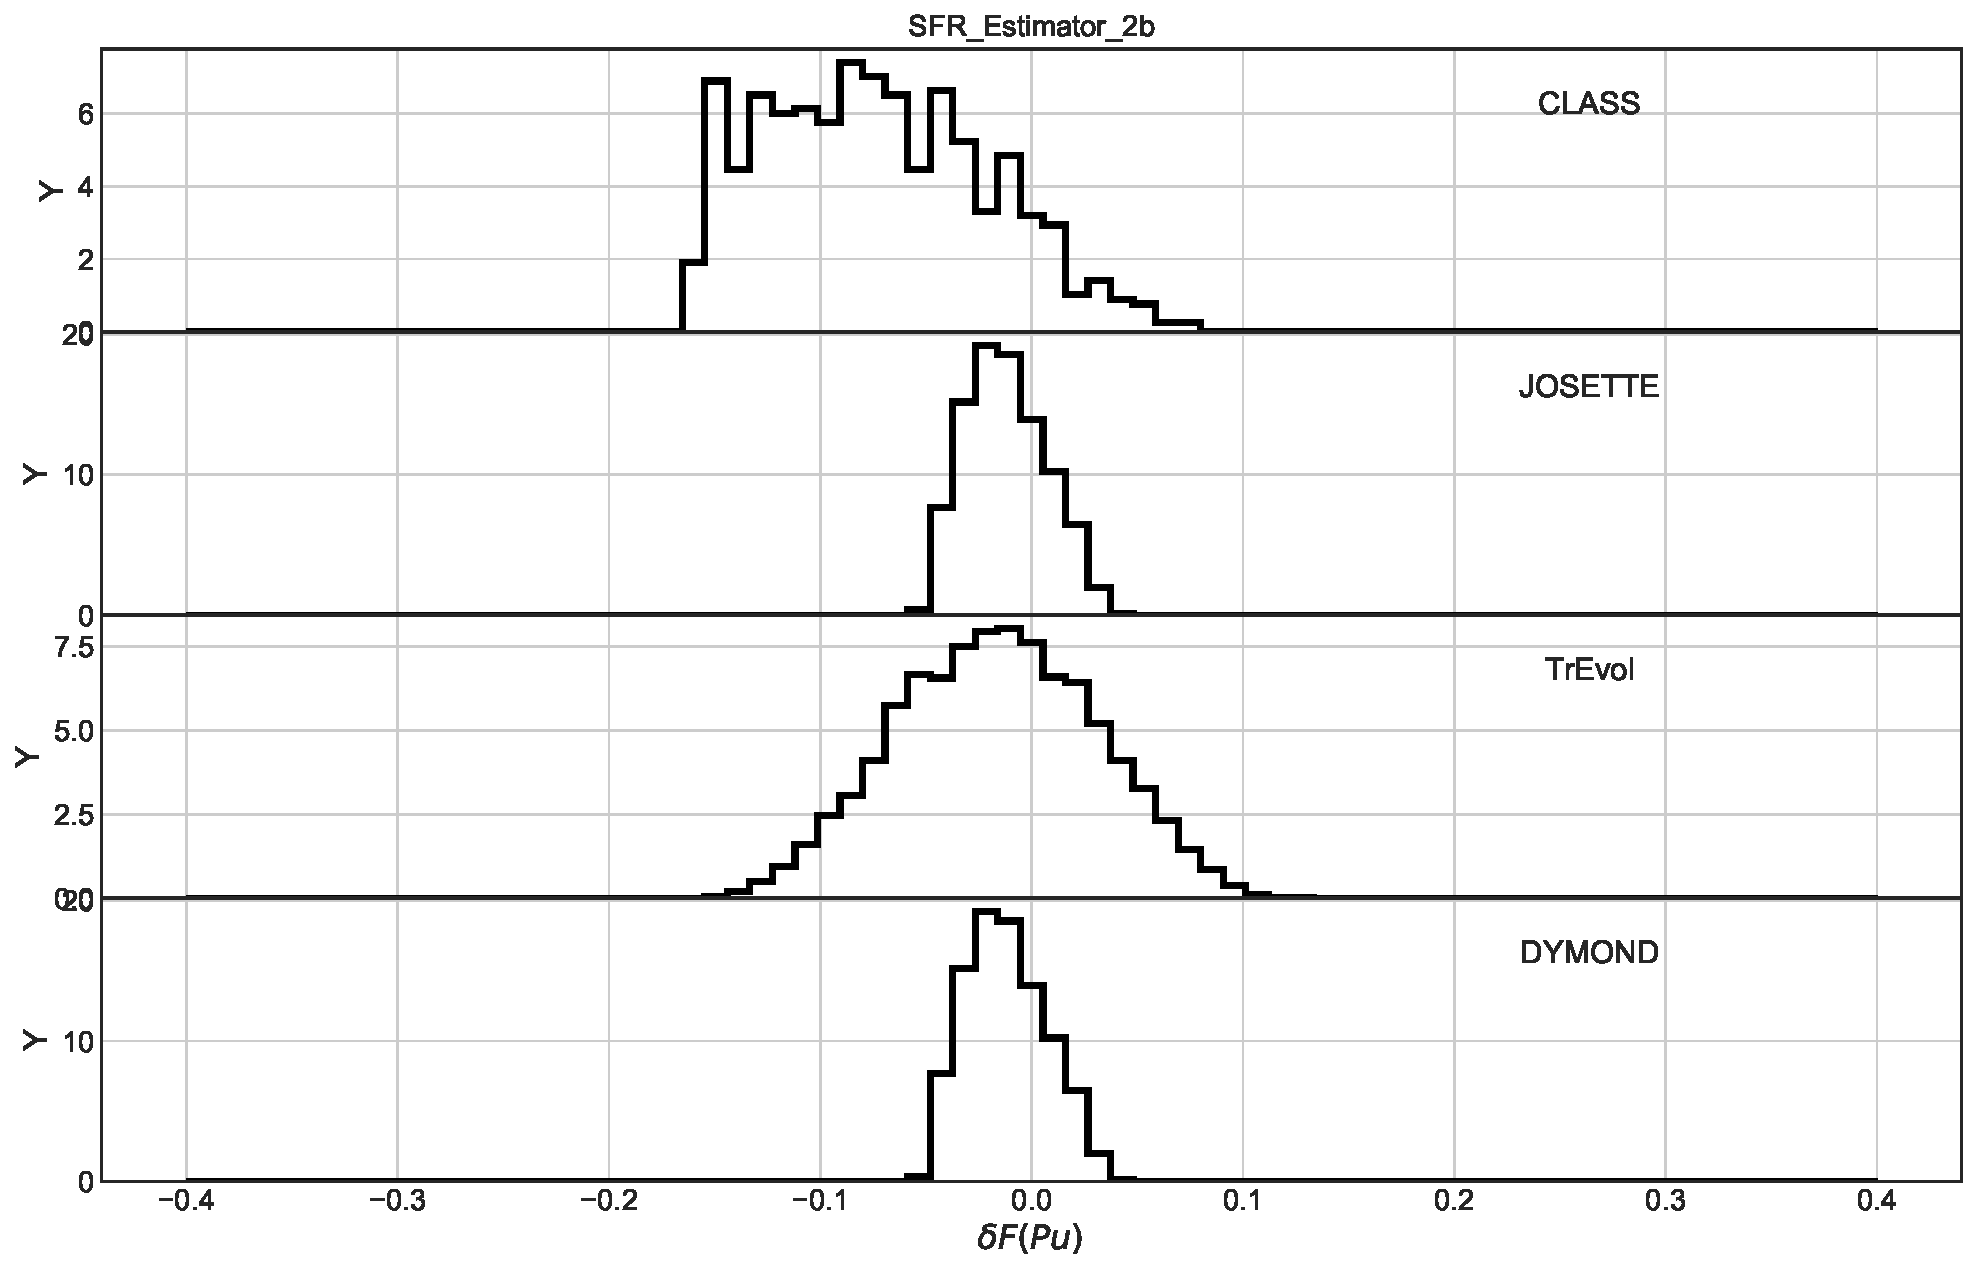
\includegraphics[width = 0.99\textwidth]{../../Feature_1/RAW_DATA/FIG/SFR_Estimator_2b.pdf}
		\caption{Estimator 2.b for SFR calculated with JOSETTE, TrEVOL, and CLASS}
		\label{fig:Est2_SFR}
	\end{center}
\end{figure}
